\section{Project Management}

The Rubin Operations plan details the operational organization. An abbreviated
description of the Rubin System is given in the document
``Vera C. Rubin Observatory System and Organization Description''
attached to the \gls{FOA}.

The \gls{USDF} is part of the Data Production department.
The department is built on teams as
depicted in \figref{fig:orgchart}. Most \gls{USDF} staff will be in the
Infrastructure team, with several in middleware and execution. These teams will have leads that report to the Associate Director for Data Production. The \gls{USDF} Infrastructure lead will be a staff member of the \gls{USDF}. The other DP
team leads are based at SLAC or NOIRLab.

It is essential that the Data Facility, whatever its host institution,
integrates with this Operations structure; see the attached description
for more details.
In particular, we emphasize that although Rubin staff are spread across multiple groups and multiple institutions, they are expected to collaborate as members of a single functional organization, working together across institutional boundaries to achieve the best outcomes for the project. This organization can be
described as a mini-matrix in Data Production. See the attached description document, section 4, Figure 8. The USDF will have an administrative structure of
its own with a point of contact that will provide advice and input to the
AD for Data Production along with similar individuals from other
data centers (see also \reqref{req:spoc} below).

\begin{figure}
\begin{center}
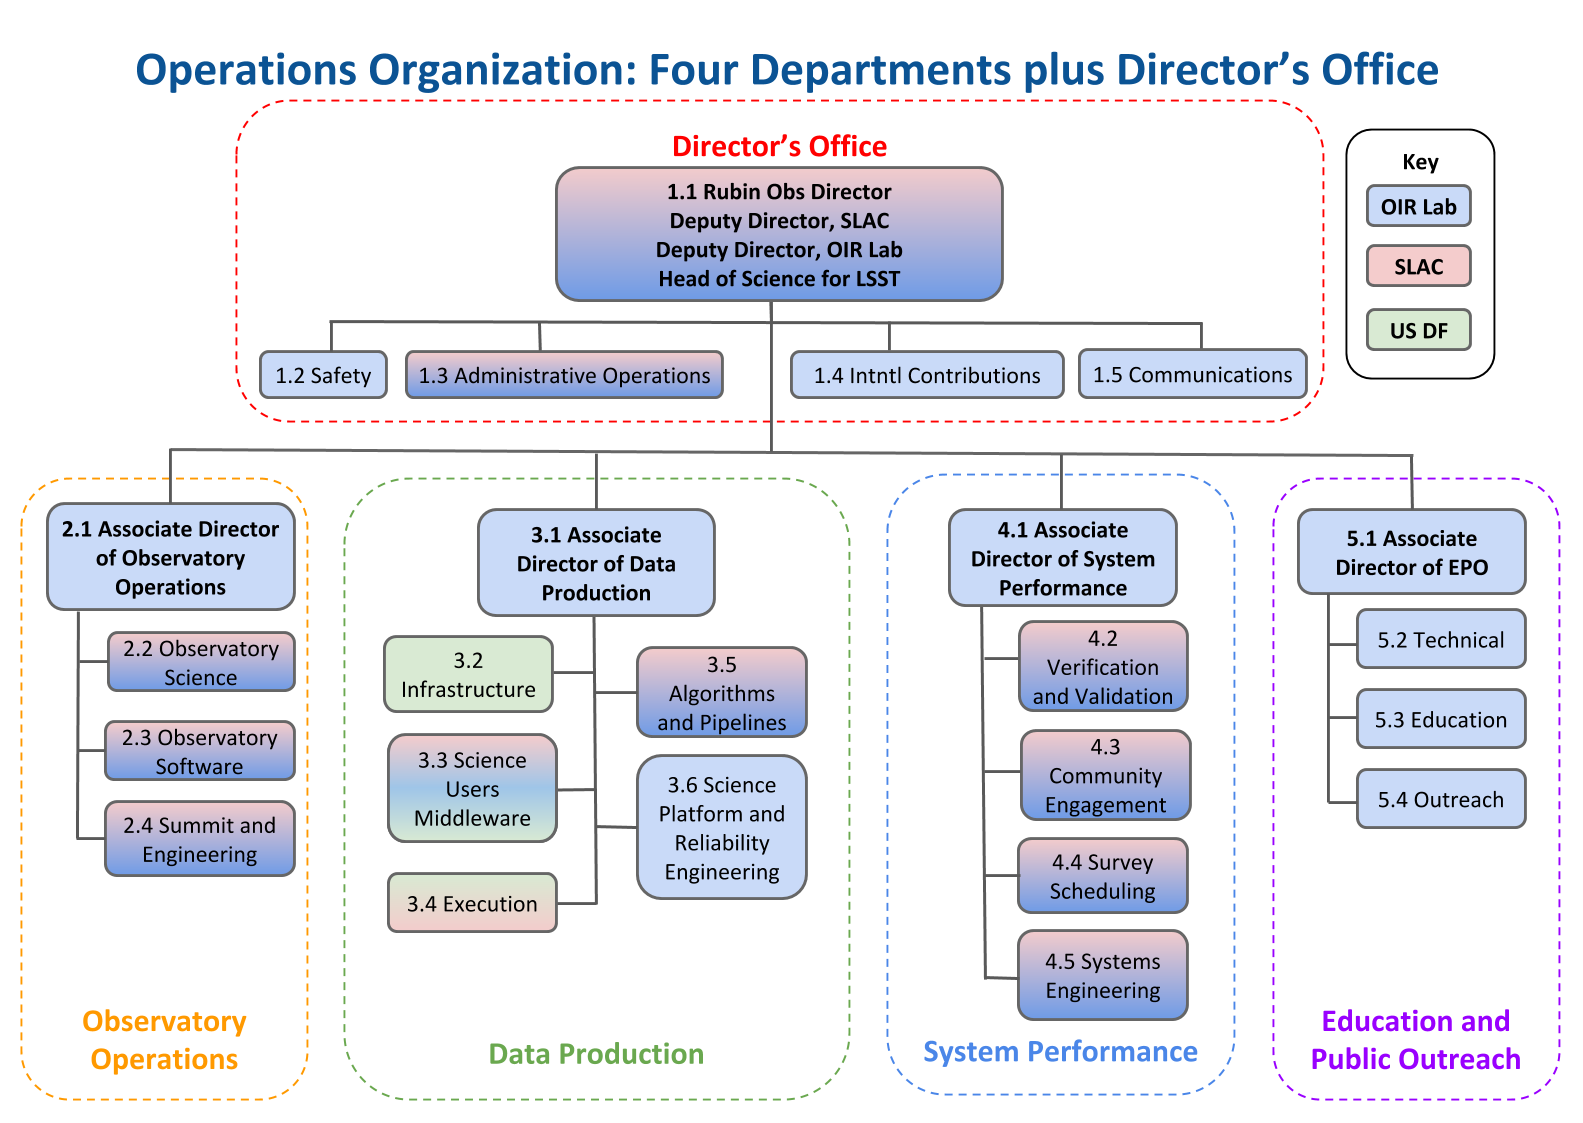
\includegraphics[width=0.8\textwidth]{figs/orgchart}
\end{center}
\caption{
The Vera Rubin Observatory Organization Chart. Shaded boxes indicate shared staff across operations partners. Staff at affiliate institutions  are included within their associated operations partner (i.e. not separately).
\label{fig:orgchart}}
\end{figure}

\newreqtype{MNGT}
\subsection{Management}\label{sec:manage}

\reqsimp{}{}{}{}{}
{
There  shall be  a the single point of contact for all managerial
aspects of the work. \label{req:spoc}
}

\reqsimp{}{}{}{}{}
{
  This work shall be carried out within the Rubin Observatory management structure under the Data Production
  department.
}

\reqsimp{}{}{}{}{}
{
The awardee shall inform Rubin Observatory management of planned changes in the
availability of staff in support of the work.
}

\reqsimp{}{}{}{}{}
{
The awardee shall conform to Rubin Observatory management practices
including use of tracking and reporting tools adopted by the observatory.
\citeds{DMTN-020} is an example of construction era practices.
}
\reqsimp{}{}{}{}{}
{The awardee will support Rubin management in all oversight committee meetings, joint agency reviews, and other management body activities as deemed necessary or desired by AURA and SLAC. 
} 

\newreqtype{PERF}
\subsection{Performance}\label{sec:perf}
\reqsimp{}{}{}{}{}
{
The awardee shall be responsible to Rubin Observatory management organizations AURA and SLAC for performance of the activities and capabilities detailed in this
SOW through a negotiated set of performance metrics. 
}
\reqsimp{}{}{}{}{}
{
The awardee's staff will receive annual performance input from Rubin management to be included in the awardee annual performance assessment process.
}

\reqsimp{}{}{}{}{}
{
Rubin management will have the authority to request that awardee staff who under perform be replaced.
}

\newreqtype{REPT}
\subsection{Reporting}
\reqsimp{}{}{}{}{}
{
The awardee shall provide a regular progress report on the status of
activities, support provided, status of anomaly investigations, etc. This
report shall cover all WPs described in this statement of and shall include
contributions from sub-contractors as appropriate. This may be integrated in
a more general Rubin Observatory report. DOE may place other, independent,
reporting requirements on the awardee.
}

\reqsimp{}{}{}{}{}
{
The frequency of reporting shall be monthly, quarterly, and annual, as
appropriate.
}

\reqsimp{}{}{}{}{}
{
Monthly reporting shall include SLA metrics to be agreed with Rubin Observatory
such as cumulative downtime, issue turn around time etc.
}

\newreqtype{COMS}
\subsection{Communications}
Regardless of funding streams, Rubin Observatory \gls{Operations} should function as one project.
While we recognize that this is not always easy for staff already embedded in another institution, it is important that we share the same tools to avoid silos and to communicate effectively about our work and to our communities.
The three primary platforms for communication at Rubin are the \gls{JIRA} ticketing system, the Slack chat system, and the web forum, community.lsst.org. Technotes are produced via LSST the Docs \citedsp{sqr-006} for Data Production. Official documentation is placed in Docushare and we also heavily use confluence. We would expect that Data Facility team members would engage with all of these.

An important part of both LSST Construction and Operations will be writing and sharing code.
All software written for \gls{LSST} is open source and publicly available, and is developed following the workflows and engineering standards described in the LSST Developer guide at \url{developer.lsst.io}.
Code developed at institutions must be developed and made available under the same conditions.


\reqsimp{}{}{}{}{}
{
\gls{USDF} staff shall use the Rubin Observatory communication tools such as JIRA, Slack and LSST the Docs.
}
\reqsimp{}{}{}{}{}
{
Any code developed for the Rubin Observatory Project shall be developed in the project repository (currently github) and shall carry the project open source license (currently \gls{GPL}).
}


\newreqtype{TRVL}
\subsection{Meetings and Travel}

\reqsimp{}{}{}{}{}
{
The awardee shall support  teleconferences  and travel in support of the
above work packages as required and agreed by both parties. At a minimum this
would include weekly video calls and in person meetings two times per year.
}

\reqsimp{}{}{}{}{}
{
The awardee shall participate in the NET group and attend the monthly telecons and meetings once or twice a year
as needed.\footnote{\url{https://confluence.lsstcorp.org/pages/viewpage.action?pageId=20284335}}
}

\newreqtype{DLVR}
\section{Deliverables}

\reqsimp{}{}{}{}{}
{
Any code deliverables shall adhere to the standards and guidelines of
Rubin Observatory as on \url{developer.lsst.io}
}
